\newpage
\section{RELATED THEORY}
\subsection{Architectural Explanations}
Image Super Resolution is a branch of Artificial Intelligence that deals with upscaling a Low-Resolution Image to High Resolution Image, filling in the missing pixels with the different techniques. There are other simpler methods to upscale images like Linear or Bi-cubic interpolation, but they do not generate any new information based on the environment and hence are not super useful to upscale an LR image. Deep Learning based methods require huge amounts of data so that the model is not overfitted, the dataset needs to contain an HR  LR version of the same image that are perfectly aligned to each other. We need to synthetically create LR images from HR images.\\
SR aims to then reverse whichever degradation process is considered, to retrieve the original underlying high-fidelity image. We have implemented SSResNet and SRGAN till now. Their architecture is explained below: 
\begin{enumerate}
    \item {\bf SRResNet:} The SRResNet is a fully convolutional network designed for 4x super-resolution. It incorporates residual blocks with skip connections to increase the optimizability of the network despite its significant depth. The SRResNet is trained and used as a standalone network and provides a nice baseline for the SRGAN – for both comparison and initialization. We use the following architecture for this network. 
    \begin{figure}[ht]
        \centering
        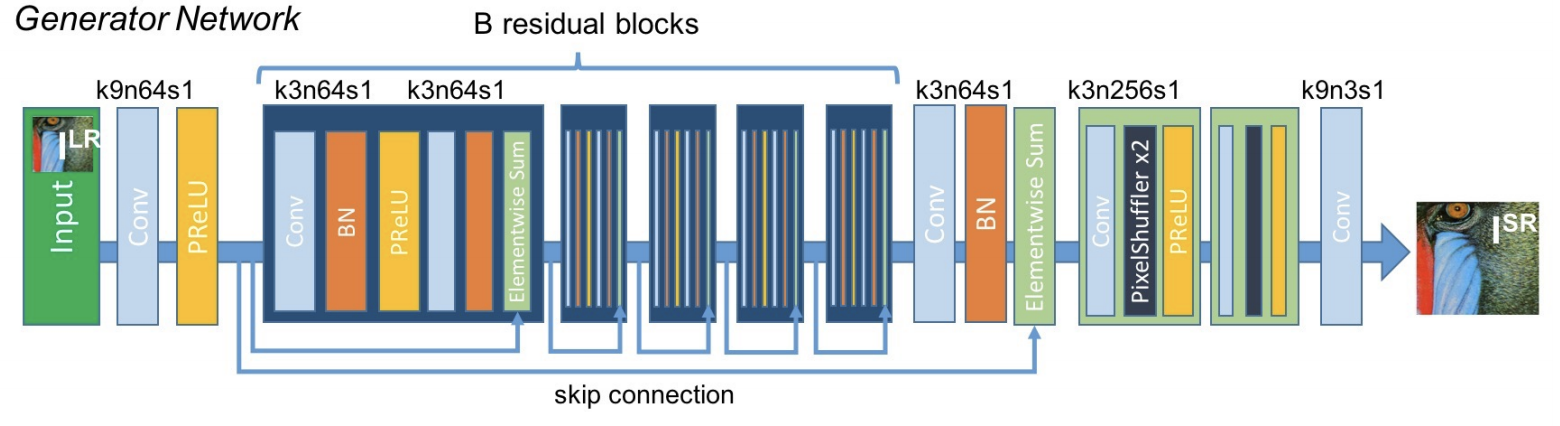
\includegraphics[width=6in]{./figures/generator.png}
        \caption{SRResNet Architecture or Generator of SRGAN}
    \end{figure} \\
    The SRResNet first contains convolution block of large Kernel Size 9x9, stride of 1 and 64 channels with PreLU activation. There are 16 residual blocks with convolution layer of Kernel size 3x3 followed by batch normalization, PreLU same conv layer again and batch normalization again. The output then is passed through same 3x3 conv layer and batch normalized. Two subpixel convolution blocks are used followed by PreLU activation each of which provides two times upscaling. Finally, a convolution with large kernel size of 9x9 and 1 stride with 3 out channels for RGB is done with Tanh activation to get super resolved image.\\ In Forward Pass, SRResNet produces a 4x upscaled image from provided low-res image using the above architecture. Mean-Squared Error (MSE) is used as the loss function to compare the upscaled image and original high-quality image. MSE is a type of content loss but here it only looks in RGB space of predicted and target images. Minimizing the MSE by changing the parameters of the network will make the model produce images closer to the original images.
    
    \item {\bf SRGAN:} Super-Resolution Generative Adversarial Network consist of two adversary networks Generator and Discriminator which are trained in tandem. The goal of the Generator is to learn to super-sample an image such that Discriminator can’t tell difference between artificial and natural origins. The interplay between these two networks leads to the improvement of both over time. \\
    The Generator learns not only by minimizing content loss, as in the case of the SRResNet but also by spying on the Discriminator's methods. By providing the Generator access to the Discriminator's inner workings in the form of the gradients produced therein when backpropagating from its outputs, the Generator can adjust its parameters in a way that alters the Discriminator's outputs in its favour. As the Generator produces more realistic high-resolution images, we use these to train the Discriminator, improving its discriminating abilities.
    \begin{figure}[ht]
        \centering
        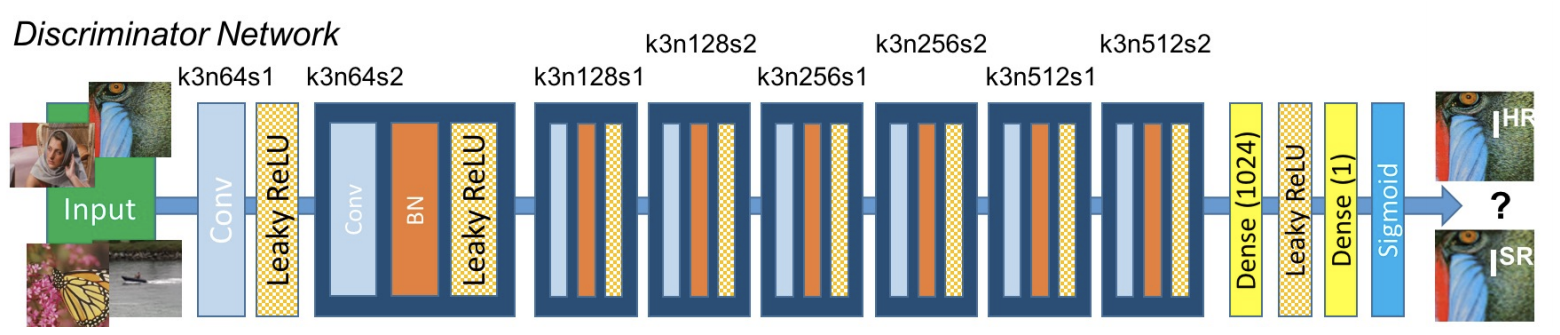
\includegraphics[width=6in]{./figures/discriminator.png}
        \caption{Discriminator Architecture}
    \end{figure} \\
    The Generator has same architecture as SRResNet. Training Discriminator is not different from any binary image classifier. It is trained on both real images and generated images from generator. In Forward Pass, it outputs the probability score $P_{HR}$. If the provided image was real, we desire the $P_{HR}$ to be as high as possible towards 1. And for generated image as low as possible towards 0. We use Binary Cross Entropy loss $-logP_{HR}$ when input image is real and $-logP_{SR}$ when image is generated. Here $P_{SR}=1-P_{HR}$. Minimizing these losses by changing the parameters will make discriminator predict higher probability for real images and lower probability for generated images.\\
    We use better content loss than that of SRResNet. In ResNet we use MSE loss in RGB space which produces overly smooth images with no finer details. There are a lot of possibilities of similar pixel combination that can be formed from low resolution image patch. When we use content loss in RGB space, it averages the output rather than choosing one of the combinations which would produce better result as an overly smooth “averaged” prediction will always have lower MSE.\\
    We can use CNN trained to classify images to find deeper meaning of patterns in images. This new representation space is more suitable for calculating content loss and can hallucinate new details showing creativity. We specifically use the VGG19 network as recommended in the paper. We use MSE-based content loss in this VGG space to compare the images. The use of content loss is only one component of the generator update, we use adversarial loss obviously. The super-resolved image is passed through the Discriminator with its weight frozen not to update the discriminator but to get the probability score $P_{HR}$ with misleading label and use the BCE loss $-logP_{HR}$ and resulting gradient information to update the Generator’s weights such that it produces images closer to its natural origin.
    GAN is trained in an interleaved fashion, where the generator and discriminator are alternatively trained for short periods of time just once before making the switch in this case.

    \subsection{General Explanations}
    \end{enumerate}
